\documentclass{amsart}

% for including graphics
\usepackage{graphicx,subcaption}

% for tikz picutures
\usepackage{tikz}
\usetikzlibrary{snakes, decorations.markings}
\tikzset{>=latex}

% for bibliography
\usepackage{biblatex}
\addbibresource{proj1.bib}

\begin{document}

\title[Math 481: Project 1]{
    Math 481, Fall 2024\medskip\\
    Project 1\\
    A funnel with variable inflow rate
}

\author{Gabriel Arteaga}
\address{Department of Mathematics and Statistics, UMBC}
\email{garteag1@umbc.edu}
\date{September 24, 2024}

\newcommand{\Maple}{\textsc{Maple}}

\begin{abstract}
We derive a mathematical model for water flowing through a
cone-shaped funnel.  Water may be added to the funnel at an
arbitrary and possibly variable rate.  Water flows out of the
funnel according to Torricelli's law.  We derive differential
equations that give the height of the water in the funnel,
and the rate of the outflow, as functions of time.  We solve
the differential equations for various inflow rates and plot
their solutions.
\end{abstract}

\maketitle

\section{Introduction}

We derive a mathematical model for the flow of water, or any
low-viscosity fluid, through a cone-shaped funnel.  Water may
be added to the funnel's open top at an arbitrarily specified
\emph{inflow rate} $Q(t)$, where $t$ is time.
The water flows out of the hole at the
funnel's bottom in accordance with
\emph{Torricelli's law}~\cite{torricelli-2,torricelli-1}.
We derive
a differential equation that describes the height $h(t)$ of
the water in the funnel as a function of time.  The equation
is not solvable in terms of elementary functions unless $Q$ is
identically zero.  We solve equation numerically in
\textsc{Maple} for various representative
inflow rates, and plot $h$ versus time.

Although $h(t)$ is determined by $Q(t)$, the two quantities
are not directly comparable because one has units of
volume per time while the other has units of length.
For a meaningful representation of the relationship
between inflow and outflow,
we derive a second differential equation that describes the
funnel's \emph{outflow rate}, $q(t)$.  We solve that differential
equation numerically for various input rates $Q(t)$, and then
plot the graphs of $Q(t)$ and $q(t)$ together for 
visual comparison.

\section{The mathematical model}

Torricelli's law states that the velocity at which fluid is ejected
from a hole at the bottom of an open-top tank filled to height
$h$ is $v = \sqrt{2gh}$, where $g$ is the acceleration due to
gravity.  Torricelli's law gives reasonably good approximation
to the outflow velocity for low viscosity fluids such as water
or gasoline, but it's not applicable at all to high viscosity
fluids, such as honey, molasses, or tar.  Our model is based on
Torricelli's Law, therefore it applies to low viscosity fluids.

We consider a funnel in the shape of the frustum of a right circular
cone with a lower radius $a$, upper radius $b$, and height $H$,
as shown in Figure~\ref{fig:schematic}.  Water flows into the
funnel's top at a volumetric rate of $Q(t)$ and leaves from
the funnel's bottom at a volumetric rate $q(t)$.
Since the area of the exit hole is $\pi a^2$, we have
\begin{equation} \label{eq:q(h)}
    q = \pi a^2 \sqrt{2gh}.
\end{equation}

\begin{figure}
	\centering
	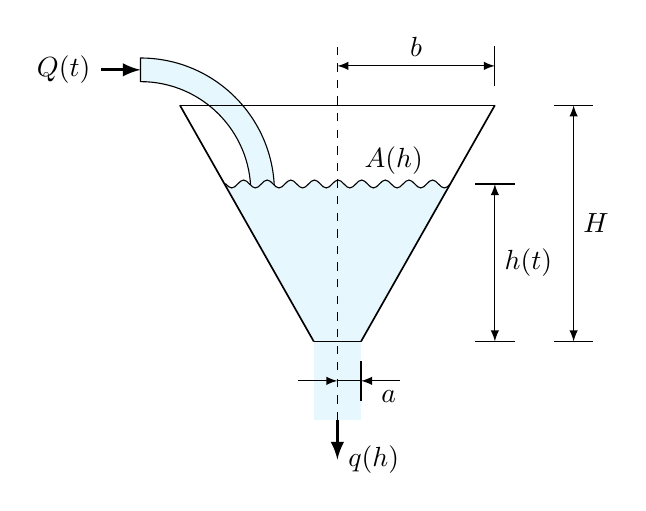
\begin{tikzpicture}[>=latex,
			snake=coil, segment aspect=0,
			segment amplitude=0.5mm, segment length=3mm]
		\pgfmathsetmacro{\H}{3}
		\pgfmathsetmacro{\a}{0.3}
		\pgfmathsetmacro{\b}{2}
		\coordinate (A) at (\a,0);
		\coordinate (B) at (\b,\H);
		\coordinate (C) at (-\a,0);
		\coordinate (D) at (-\b,\H);
		\coordinate (E) at (intersection of A--B and -10,2 -- 10,2);
		\coordinate (F) at (intersection of C--D and -10,2 -- 10,2);
		\coordinate (U) at (0,-0.5);
		\path (B -| 0,0) +(0, 0.5) coordinate (V);	% define point (V)
		\coordinate (W) at (0,2);
		\coordinate (hfoot) at (2,0);
		\coordinate (Hfoot) at (3,0);

		% inflow
		\begin{scope}[shift={(-2.5,3.3)}]
			\draw[->,very thick] (-0.5,0.15) node[left] {$Q(t)$} -- (0,0.15);
			\draw[fill=cyan!10] (0,0) arc (90:0:1.4) -- +(0.3,0)
		  		arc (0:90:1.7) -- cycle;
		\end{scope}

		% funnel contents
		\fill[cyan!10] (A) -- (E) [snake=coil] -- (F) [snake=none] -- (C);

		% outflow
		\fill[cyan!10] (A) +(0,-1) rectangle (C);
		\draw[->, very thick] (0,-1) -- +(0,-0.5) node[right] {$q(h)$};

		% the funnel
		\draw[semithick] (A) -- (B)  (C) -- (D);
		\draw (A) -- (C)  (B) -- (D);

		% the b marker
		\draw[<->] (V) -- (V -| B) node[pos=0.5, above] {$b$};
		\draw (V -| B) +(0,-0.25) -- +(0,0.25) coordinate (X);

		% the a marker
		\draw[->] (U) +(-0.5,0) -- (U);
		\draw (U) -- (U -| A);
		\draw[<-] (U -| A) -- +(0.5,0) node[pos=0.7, below] {$a$};
		\draw (U -| A) +(0,-0.25) -- +(0,0.25);

		% the h(t) marker
		\draw[<->] (hfoot) -- (hfoot |- W) node[pos=0.5,right] {$h(t)$};
		\draw (hfoot) +(-0.25,0) -- +(0.25,0);
		\draw (hfoot |- W) +(-0.25,0) -- +(0.25,0);

		% the H marker
		\draw[<->] (Hfoot) -- (Hfoot |- B) node[pos=0.5,right] {$H$};
		\draw (Hfoot) +(-0.25,0) -- +(0.25,0);
		\draw (Hfoot |- B) +(-0.25,0) -- +(0.25,0);

		% water level
		\draw[snake] (E) -- (F) node[pos=0.25, above] {$A(h)$};

		% funnel axis
		\draw[dashed, very thin] (0,-1) -- (0,-1 |- X);
	\end{tikzpicture}

    \caption{
        Water flows into the funnel at the volumetric rate of $Q(t)$
        and flows out at speed $\sqrt{2gh(t)}$.
        The area $A\bigl(h(t)\bigr)$ of the water's exposed surface
		varies with the water level~$h(t)$ in the funnel.
    }
	\label{fig:schematic}
\end{figure}

Let $V=V(t)$ be the volume of the water in the funnel at time~$t$.
The rate of change of $V$ equals the rate of inflow minus the rate of
outflow:
\[
    \frac{dV}{dt} = Q(t) - \pi a^2 \sqrt{2gh}.
\]
We know from calculus that
$dV = A(h) \, dh$ where $A(h)$ is the funnel's horizontal cross-sectional
area at level~$h$.  Therefore $dV/dt = A(h) \, dh/dt$ and the previous
equation changes to:
\begin{equation} \label{eq:de}
    A(h) \frac{dh}{dt} = Q(t) - \pi a^2 \sqrt{2gh}.
\end{equation}
It remains to obtain an expression for~$A(h)$.

Toward that end, let $r(h)$ be the radius of the funnel's
horizontal cross-section at a height~$h$ above the bottom.
In Figure~\ref{fig:funnel-cross-section}
we see a vertical cross-section of the funnel.
%
\begin{figure}
    \centering
	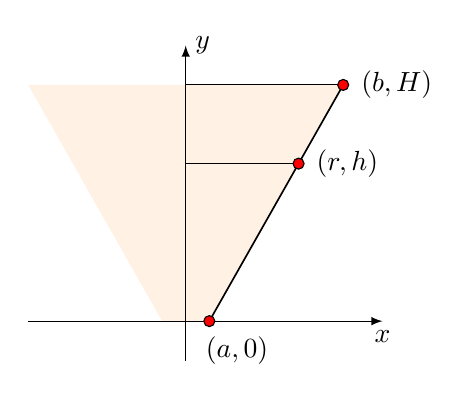
\begin{tikzpicture}
		\pgfmathsetmacro{\H}{3}
		\pgfmathsetmacro{\a}{0.3}
		\pgfmathsetmacro{\b}{2}
		\coordinate (A) at (\a,0);
		\coordinate (B) at (\b,\H);
		\coordinate (C) at (-\a,0);
		\coordinate (D) at (-\b,\H);
		\coordinate (E) at (intersection of A--B and -10,2 -- 10,2);
		\coordinate (U) at (0,-0.5);
		\path (B -| 0,0) +(0, 0.5) coordinate (V);	% define point (V)

		\fill[orange!10] (A) -- (B) -- (D) -- (C) -- cycle;

		% the coordinate axes
		\draw[->] (-2,0) -> (2.5,0) node[below] {$x$};
		\draw[->] (U) -> (V) node[right] {$y$};
		
		\draw[semithick] (A) -- (B);
		\draw (B) -- (B -| 0,0);
		\draw (E) -- (E -| 0,0);
		
		\draw[fill=red] (A) circle (0.07) +(1em,-2.5ex) node {$(a,0)$};
		\draw[fill=red] (B) circle (0.07) node[right=0.3em] {$(b,H)$};
		\draw[fill=red] (E) circle (0.07) node[right=0.3em] {$(r,h)$};

	\end{tikzpicture}

    \caption{
        The diagram represents a vertical cross-section of the funnel
		through its axis or symmetry.
        The points with coordinates $(b,H)$ and $(a,0)$
		lie on the top and bottom rims, while 
		$(r,h)$ is an arbitrary point along the line that connects those
		points.
    }
	\label{fig:funnel-cross-section}
\end{figure}
%
The ``edge'' of
the funnel is represented by the slanted line that connects the points
with coordinates $(a,0)$ and $(b,H)$.  The equation of that line is:
\[
    y = \frac{H}{b-a} (x-a).
\]
To find the radius at level $r$, we plug in $y=h$ and solve for $x$
which gives the desired~$r(h)$ as
\begin{equation} \label{eq:r(h)}
    r(h) = a + \frac{b-a}{H} h.
\end{equation}
We note that this equation implies that $r(0) = a$ and $r(H)=b$, as expected.

In equation~\eqref{eq:de}
we replace the area $A(h)$ with $\pi r(h)^2$, where $r(h)$ is as
in~\eqref{eq:r(h)}, and arrive at
\begin{equation} \label{eq:de-expanded}
    \pi \Bigl[ a + \frac{b-a}{H} h \Bigr]^2 \frac{dh}{dt} =
        Q(t) - \pi a^2 \sqrt{2gh}.
\end{equation}
This first order differential equation,
together with an initial condition $h(0)=h_0$, yields the height $h(t)$
of the water in the funnel at all future times.
The solution is \emph{not} expressible in terms of elementary functions
in general.  In the subsequent sections
we resort to \textsc{Maple} to solve it numerically
and plot the graphs of $h(t)$.

\section{Constant inflow rate}
\label{sec:Constant Inflow Rate}
In the rest of this article we will use the following parameters
for the funnel's geometry and the acceleration of gravity:
\[
    a = 1, \quad
    b = 7, \quad
    H = 10, \quad
    g = 1.
\]
We also assume that the funnel is initially full to the brim,
that is, $h(0)=H$.

The choice of $g=1$ is not as strange as it may seem.  After all,
the numerical value of $g$ depends on the units of measurement.
For instance,
$g$ is $9.81~\mathrm{m/sec^2}$
in one system of measurements, and
$32~\mathrm{ft/sec^2}$ in another.
In our computations we assume
a system of measurements in which $g=1$.
Of course any other positive number will do equally well.

Figure~\ref{fig:h-vs-t} shows the graphs of $h(t)$
for three different choices of $Q(t)$.  The leftmost graph
corresponds to no inflow.  We see that the water level drops
to zero in finite time.  The two other graphs correspond to
constant inflow rates of $Q=6$ and $Q=10$.  We see that in
each case the water level stabilizes to a fixed level after
sufficiently long wait.

\begin{figure}
    \centering
    \includegraphics[width=0.32\textwidth]{h-1.png}
    \includegraphics[width=0.32\textwidth]{h-2.png}
    \includegraphics[width=0.32\textwidth]{h-3.png}
    \caption{
        The three graphs of $h$ versus $t$ correspond
        to the constant input rates of
        $Q(t) = 0$, 
        $Q(t) = 6$, 
        $Q(t) = 10$, 
        respectively.  Note that the horizontal axes
        are scaled quite differently.
    }
	\label{fig:h-vs-t}
\end{figure}

We ask: \emph{What determines the stabilization level?  That is, what is
the horizontal asymptote of $h(t)$ corresponding to
a constant inflow rate $\bar{Q}$?}

It turns out that the answer may be obtained with simple
algebra.  To see this, note that as
$h(t)$ approaches its horizontal asymptote, then its slope, that is
$dh/dt$, goes to zero.  Looking at the differential
equation~\eqref{eq:de-expanded}, we see the left hand side goes
to zero, therefore the right hand size will have to go to zero too.
Setting the right hand size to zero and solving for $h$ we
obtain the asymptotic value, $h_\infty$:
\[
    h_\infty
	= \lim_{t\to\infty} h(t)
	= \frac{1}{2g} \Bigl( \frac{\bar{Q}}{\pi a^2}  \Bigr)^2.
\]

For example, with the previously used parameter values of $a=1$,
$g=1$ and $\bar{Q}=10$, we get $h_\infty \approx 5.066$
which agrees with the
asymptotic limit of the rightmost graph in
Figure~\ref{fig:h-vs-t}.

\section{Variable inflow rate}

In this section we present two examples where the inflow rates vary with time.

\subsection{Multistep inflow rate}
\label{subsec:step-input}

We take:
\[
    Q(t) = \begin{cases}
        2  &  \text{if } 0< t<60, \\
        9  &  \text{if } 60<t<150,\\
        6  &  \text{if } t > 150.
    \end{cases}
\]

The graphs of $Q(t)$ and the corresponding $h(t)$ are shown
in Figure~\ref{fig:step-input}.

\begin{figure}
    \centering
    \includegraphics[width=0.4\textwidth]{input-piecewise.png}
    \includegraphics[width=0.4\textwidth]{h-piecewise.png}
    \caption{
        On the left is the inflow rate versus time.
        On the right is the corresponding water level, $h(t)$, versus time.
    }
	\label{fig:step-input}
\end{figure}

\subsection{Sinusoidal inflow rate}
\label{subsec:sine-input}

We take:
\[
    Q(t) = 7 + 1.5 \sin \frac{1}{20} t.
\]

The graphs of $Q(t)$ and the corresponding $h(t)$ are shown
in Figure~\ref{fig:sinosoidal-input}.

\begin{figure}
    \centering
    \includegraphics[width=0.4\textwidth]{input-sine.png}
    \includegraphics[width=0.4\textwidth]{h-sine.png}
    \caption{
        On the left is the inflow rate versus time.  On the right is the 
        corresponding water level, $h(t)$, versus time.
    }
	\label{fig:sinosoidal-input}
\end{figure}

\section{The critical flow rate}
\label{sec:critical flow rate}

We define the funnel's \emph{critical flow rate}, $Q_\text{cr}$, as the
constant rate of inflow that keeps the funnel full to the brim
without overflowing.
\\
As flow rate is constant then rate of change of volume is $0$, inclusively our height will stay at $H$. This gives the expression
\begin{align*}
    0=\frac{dV(t)}{dt}= Q_{\text{cr}} - \pi a^2 \sqrt{2gH}\\
    \text{Using our parameters from \ref{sec:Constant Inflow Rate}}\\
    0=Q_{\text{cr}} - \pi \sqrt{20} \\
     Q_{\text{cr}}= \pi \sqrt{20}
\end{align*}
Thus our \emph{critical flow rate} comes out to $ \pi \sqrt{20}$. 

\section{Comparing the inflow and outflow rates}

The two graphs in Figure~\ref{fig:step-input} are not directly comparable
since one depicts the \emph{inflow rate} and the other the \emph{water level}.

\begin{quotation}
    \emph{To do:}
	Derive a differential equation for the funnel's outflow rate $q(t)$.
	Solve the equation for the inputs given in
	subsections~\ref{subsec:step-input} and~\ref{subsec:sine-input}.
	In each case plot $Q(t)$ and $q(t)$ together in one coordinate system.
\end{quotation}
We begin recalling the definition of $q(t)$ equation \ref{eq:q(h)},
\[q(t)=\pi a^2 \sqrt{2gh(t)}\]
From this we can find an alternate equation for $h(t)$,
\[h(t)=\frac{q(t)^2}{2\pi^2 a^4 g}\]
Using this alternate definition we can attain a differential equation for $q(t)$ by using~\eqref{eq:de-expanded},
\[
    \frac{d}{dt}q(t)=
    \frac{(Q-q(t))a^4g}{q(t)}
\]
Using our parameters from \ref{sec:Constant Inflow Rate}, we can define 2 different cases. One where 
\[
Q(t)= 7 + 1.5 \sin \frac{1}{20} t,
\text{ and } 
Q(t)=\begin{cases}
        2  &  \text{if } 0< t<60, \\
        9  &  \text{if } 60<t<150,\\
        6  &  \text{if } t > 150.
    \end{cases}
    \]
For the first case we arrive at 
\[
\frac{d}{dt}q(t)=
    \frac{(7+1.5(\sin(\frac{t}{20})-q(t))}{q(t)}.
\]
For the second case we arrive at
\[
    \frac{d}{dt}q(t)=
    \frac{\left(\begin{cases}
        2  &  \text{if } 0< t<60, \\
        9  &  \text{if } 60<t<150,\\
        6  &  \text{if } t > 150.
    \end{cases}
    -q(t)\right)}{q(t)}.
\]
The graphs of each are located in the page below.
\begin{figure}
    \centering
    \includegraphics[width=0.7\linewidth]{proj1piecewisegraph10.png}
    \includegraphics[width=0.7\linewidth]{proj1sinegraph10.png}
    \caption{
    The above graphs show the comparison of $Q(t)$ (in blue) and $q(t)$ (in red) over a time interval of $t=0$ to $t=400$. Piece-wise case on top and sinusoidal case on bottom.}
    \label{fig:enter-label}
\end{figure}
\printbibliography

\end{document}

